\documentclass{article}
\author{Thibault Gelly\\
        William Le Gavrian}
\title{Programmation Orientée Objet - Projet Puissance 4}

\usepackage{graphicx}
\graphicspath{ {./images/} }

\begin{document}
\date{}
\maketitle
\tableofcontents

\section{Introduction}

L'objectif de ce projet est de réaliser un jeu "Puissance 4" en Java.
La grille de jeu est représentée par une matrice doublement chaînée.
Le cahier des charges du jeu est le suivant :

\begin{itemize}
  \item Le jeu doit proposer un affichage propre dans un terminal en utilisant les caractères unicodes et les codes
  d'échappement ANSI.
  \item La vérification de victoire doit se faire récursivement pour exploiter les avantages de la matrice doublement chaînée.
  \item Le joueurs peuvent spécifier leurs noms et choisir la couleur avec laquelle ils veulent jouer.
  \item Une partie peut être sauvegardée dans un fichier, et les joueurs peuvent par la suite charger la partie sauvegardée et 
  la continuer.
\end{itemize}

\section{Vue d'ensemble du programme}

\begin{figure}
  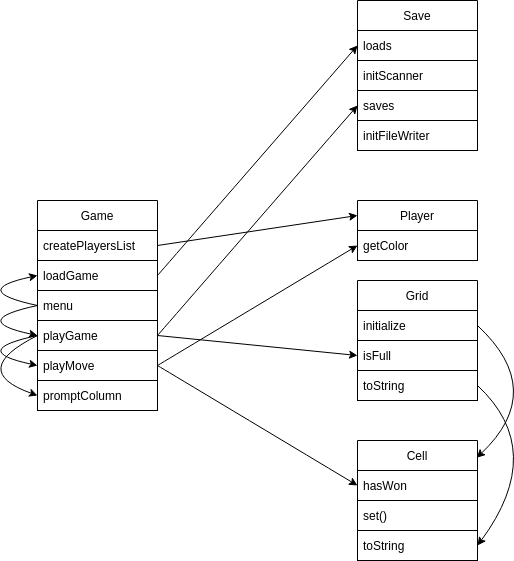
\includegraphics[width=12cm]{diagram.png}
  \centering
  \caption{UML du programme.}
\end{figure}

La figure ci-dessus montre les interactions entre les différentes classes du programme. Chaque flèche correspond à un appel de
fonction.

Le programme remplit le cahier des charges :

\begin{itemize}
  \item L'affichage se fait dans le terminal et est dynamique :
  Après chaque coup, on efface la grille affichée précédemment, puis on la réaffiche en ayant ajouté le nouveau coup.
  \item Lorsqu'un coup est joué, on part de la position de ce coup pour tester s'il permet d'aligner quatre jetons ou pas. Cette
  vérification se fait de manière récursive dans toutes les directions: diagonale haut-droite, vers la droite, diagonale bas-droite, 
  vers le bas, diagonale bas-gauche, vers la gauche et diagonale haut-gauche.
  \item Pour l'affichage, on propose à l'utilisateur de choisir une couleur en début de partie. Pour cela, on a récupéré les codes
  unicode des émojis de chaque couleur (sauf le blanc qui sert pour les cases vides). Chaque joueur choisit également un nom qui
  sera utilisé lorsqu'il doit jouer un coup ou lorsqu'il gagne la partie.
  \item La sauvegarde est opérationnelle : Si une partie est terminée ou si l'utilisateur entre la lettre q (pour quit) à la place
  d'un numéro de colonne, en choisissant de charger un fichier à la prochaine exécution, on verra s'afficher tous les coups de la partie
  précédemment jouée un par un. Ensuite, si la partie n'était pas terminée, on pourra la continuer.
\end{itemize}

\section{Le code}

Dans cette section, on détaille le code. Chaque sous-section correspond à une classe Java et décrit son fonctionnement. Les classes
sont présentées ici dans le même ordre que nous les avons développées, c'est à dire de l'élément atomique (la cellule) vers l'objet
plus global (la partie).

\subsection{Cell}

Cell est une classe qui encapsule une cellule d'une matrice doublement chaînée. Une cellule a quatre références sur des cellules qui
sont associées à ses voisins s'ils existent. Elle a également un champs value qui contient le code unicode qui correspond à un émoji
de couleur. Si la case est vide, cet émoji est blanc.

\subsection{Grid}

Grid est une classe qui encapsule une matrice doublement chaînée.
Le maillon upperLeftCorner est celui qui se situe en haut à gauche de la grille. C'est à partir de ce maillon que la fonction
initialize() crée toute la grille. Au début, nous avons eu des difficultés avec la matrice doublement chaînée, et nous avons implémenté
la grille avec un tableau de cellules. Par la suite, nous avons compris comment initialiser une matrice doublement chaînée, et nous avons
écrit l'implémentation finale.

\subsection{Game}

La classe Game encapsule tout le programme. Sa fonction menu() est appelée par le Main, et elle permet à l'utilisateur de choisir si
il veut jouer une nouvelle partie ou en charger une ancienne. Ensuite, c'est la fonction playGame() ou loadGame() qui prend le relais.

\subsection{Player}

La classe Player n'a aucune méthode, elle encapsule simplement les données d'un joueur : son numéro, son nom et la couleur qu'il joue.
L'avantage structurel d'encapsuler ces données dans une classe réside dans l'appel de la fonction playMove(). Sans cette classe Player, 
il aurait fallu passer en paramètres de playMove() un identifiant permettant de touver les informations du joueur, par exemple dans un
tableau ou un dictionnaire. Cette classe a donc pour principale utilité d'améliorer la lisibilité du code.

\subsection{Save}

Save est une classe qui met à disposition de Game des fonctions qui permettent d'écrire ou de lire des données dans un fichier save.txt.
Il s'agit ici d'une sauvegarde par action et non pas par état : on sauvegarde une ligne pour chaque coup joué. Cela signifie que pour 
rejouer la partie contenue dans un fichier, il faut obligatoirement le lire ligne par ligne pour obtenir l'état final de la partie
enregistrée. Les données d'un coup joué sont stockées sous ce format : \{n° de joueur\}/\{colonne du coup joué\}. On stocke un coup de
cette manière à chaque ligne du fichier save.txt.

\end{document}